\documentclass{beamer}
\usepackage{lmodern}

% \setbeameroption{show notes}
% \setbeameroption{show notes on second screen=⟨location⟩} % left, bottom, top
% \setbeameroption{show only notes}

\usepackage[utf8]{inputenc}
\usepackage{graphicx}
\usepackage{csvsimple}

\usepackage{amsfonts, amsmath, amssymb, amstext}		% AMS-Paket
\DeclareMathOperator*{\argmin}{arg\,min}
\DeclareMathOperator*{\argmax}{arg\,max}
\usepackage{siunitx}
\usepackage{varwidth}


\DeclareSIUnit\dbm{\decibel{}m}

% Druckanpassung zur Darstellung mehrerer Folien auf einer A4 Seite
% \usepackage{pgfpages}
% \pgfpagesuselayout{4 on 1}[a4paper, border shrink=5mm, landscape] % landscape ist Querformat

\usetheme{Antibes} % Auskommentieren, um Druckerschwärze zu sparen
\usecolortheme{lily}
\useinnertheme{circles}
\beamertemplatenavigationsymbolsempty % Symbole unten rechts ausblenden
\setbeamertemplate{footline}[frame number] % Foliennummerierung
\setbeamertemplate{sections in toc}[sections numbered]
\setbeamertemplate{subsection in toc} {\leavevmode\leftskip=1em$\bullet$\hskip1em\inserttocsubsection\par}
 \renewcommand{\arraystretch}{1.5}
 \usepackage{subcaption}					% Untergraphiken erstellen

\renewcommand\textbullet{\ensuremath{\bullet}}

\makeatletter
\def\beamer@sectionintoc#1#2#3#4#5{%
  \ifnum\c@tocdepth>0%
  \ifnum#4=\beamer@showpartnumber%
  {
  \beamer@saveanother%
  \gdef\beamer@todo{}%
  \beamer@slideinframe=#1\relax%
  \expandafter\only\beamer@tocsections{\gdef\beamer@todo{%
      \beamer@tempcount=#5\relax%
      \advance\beamer@tempcount by\beamer@sectionadjust%
      \edef\inserttocsectionnumber{\the\beamer@tempcount}%
      \def\inserttocsection{\hyperlink{Navigation#3}{#2}}%
      \beamer@tocifnothide{\ifnum\c@section=#1\beamer@toc@cs\else\beamer@toc@os\fi}%
      {
        \ifbeamer@pausesections\pause\fi%
        \ifx\beamer@toc@ooss\beamer@hidetext
          \vskip1.0em
        \else
          \vskip1em%HIER EINSTELLEN
        \fi
        {%
          \hbox{\vbox{%
              \def\beamer@breakhere{\\}%
              \beamer@tocact{\ifnum\c@section=#1\beamer@toc@cs\else\beamer@toc@os\fi}{section in toc}}}%
         \par%
        }%
      }%
    }
  }%
  \beamer@restoreanother%
  }
  \beamer@todo%
  \fi\fi%
}
\makeatother


\title[Style-Specific Beat Tracking with DNNs]{Style-Specific Beat Tracking with \\Deep Neural Networks}
\subject{} % pdf-Dateieigenschaften
% \author[Julius Richter]{Julius Richter}
\author{Julius Richter \texorpdfstring \newline \texorpdfstring \newline \tiny julius.marius.richter@googlemail.com \texorpdfstring \newline \texorpdfstring \url{https://github.com/julius-richter/beat\_tracker}}

\institute{Technische Universität Berlin\\ Audio Communication Group}
% \logo{\includegraphics[width=0.7cm]{figures/TU-Berlin-Logo.eps}}
% \date
\date{\today}
\keywords{FSO}


\begin{document}


\maketitle


\begin{frame}
\frametitle{Overview}
\tableofcontents
% \tableofcontents[sections={1-6},hideallsubsections]	
\end{frame}


% Berrou introduced Turbo-codes as a new class of convolutional codes 
% Performance in terms of BER is close to the Shannon limit
% Turbo encoder is built using a parallel concatenation of tho Recursive Systematic Concolutional codes
% Decoder is using a feedback decoding rule  


\section{Introduction}

\begin{frame}
\frametitle{What is Beat Tracking?}
\begin{minipage}{\textwidth} 
\centering
\includegraphics[scale=0.6]{figures/audio.pdf}
\end{minipage}
\hfill
\begin{itemize}
\item \textbf{Intuition}: Recovering a sequence of time positions from a musical input that are consistent with the times when a human might tap their foot.
\item \textbf{Beat}: \emph{Phenomenal experience} of perceived pulses, which are approximately equaliy spaced, and define the rate at which notes in a piece of music are played (in Western music often designated as quarter notes) \cite{Handel1989}.
% \item Automatic analysis of the temporal structure in an audio piece
\item Computational method: Initial step in the computer emuation of human music understanding.
\end{itemize}
\end{frame}



\begin{frame}
\frametitle{Difficulties of Beat Tracking}
\centering
\fbox{\parbox{21em}{\centering Problem of inferring an original beat structure that is not expressed explicitly in the audio signal}}
\vfill
\begin{itemize}
\item Audio signals consist of sounds of various kinds of instruments and other sound sources
\item Beats may not directly correspond to a real sound
\item Soft onsets, heavy syncopation, and expressive timing
\item Blurred note transitions, and the absence of a clear rhythmic structure (e.g. in classical music)
\item Multiple interpretations of the beat structure are possible
\end{itemize}
\end{frame}




\begin{frame}
\frametitle{Applications of Beat Tracking}
\centering
\fbox{\parbox{21em}{\centering Automate time-consuming tasks \\ in order to synchronize events with music}}
\vfill
\begin{itemize}
\item Audio and video editing 
\item Stage light control in live performances
\item Automatic indexing and content-based retrieval of audio data
\item Temporal segmentation for higher-level MIR tasks such as chord estimation, harmonic description, automatic transcription and score extraction from performance data 
\item Automatic playlist generation
\item Synchronization of a musical performance with computers or other devices (MIDI clock)
\end{itemize}
\end{frame}



\begin{frame}
\frametitle{Goals of the Thesis}
\begin{itemize}
\item Naive approach: Specify an accurate list of onset times and estimate the beat positions as the predominant periodicity 
\item Method lacks abstraction, and using hand-crafted features or heuristics lead to a proliferation of rules and exceptions
\item[$\Rightarrow$] Adapt a machine learning approach: \emph{supervised learning} with a large training set of various musical pieces $\mathbf x$ with annotated beats as targets $\mathbf y$
\begin{align}
\hat{\mathbf y} = f_{\boldsymbol \theta}(\mathbf x)
\end{align} 
\item Reimplementation of a current state-of-the-art beat tracker \cite{Boeck2014} based on recurrent LSTM networks $\rightarrow$ slow in training 
\item Use a convolutional approach: Influenced by the good results in audio synthesis (Google WaveNet \cite{Oord2016})

\end{itemize}


\end{frame}




\section{Beat Tracking System}

\begin{frame}
\frametitle{Beat Tracking System}
\begin{minipage}{\textwidth} 
\centering
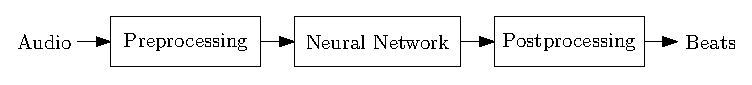
\includegraphics[scale=0.75]{figures/beat_tracking_system.eps}
\end{minipage}
\vfill
\begin{minipage}{\textwidth} 
\centering
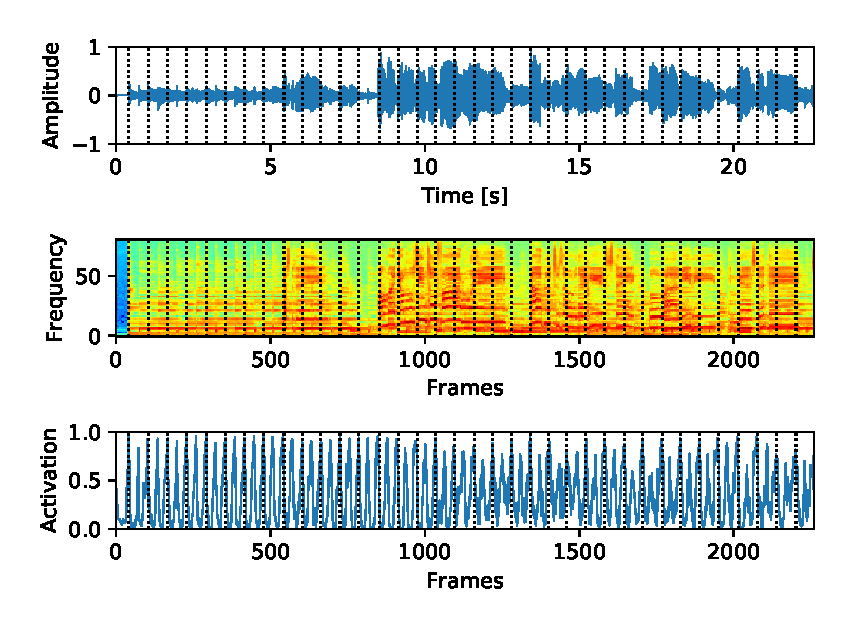
\includegraphics[scale=0.5]{figures/pipeline.eps}
\end{minipage}

\end{frame}


\begin{frame}
\frametitle{Compound Dataset}
\begin{itemize}
\item The dataset comprises a wide range of different musical styles
(Blues, Cha-Cha-Chá, Choral, Classical, Country, Disco, Folk, Hip-hop, Jazz, Jive, Metal, Pop, Quickstep, Reggae, Rock, Rumba, Samba, Tango, and Waltz)
\end{itemize}
\begin{table}[htbp]
\centering
\footnotesize
\begin{tabular}{lrrr}
\hline
\hline
\textbf{Dataset} & \textbf{Files} & \textbf{Length} & \textbf{Beats} \\
\hline
Ballroom \cite{Gouyon2006b, Krebs2013} & $685$ & $5\,\text{h} \;57\,\text{m}$ & $\num{44653}$\\
GTZAN \cite{Tzanetakis2002b, marchand2015swing} & $1000$ & $8\,\text{h}\;20\,\text{m}$ & $\num{59277}$\\
Hainsworth \cite{Hainsworth2004} & $222$ & $3\,\text{h}\;19\,\text{m}$ & $\num{22339}$\\
SMC \cite{Holzapfel2012} & $217$ & $2\,\text{h}\;25\,\text{m}$ & $\num{10628}$\\    
\hline
Total & $2124$ & $ 20\,\text{h}\; 01\,\text{m}$ & $\num{136897}$\\  
\hline
\hline
\end{tabular}
\end{table}  

\end{frame}


\subsection{Data Preprocessing}

\begin{frame}
\frametitle{Data Preprocessing}
\begin{itemize}
\item Resample at rate $f_s = 44.1 \,\text{kHz}$ with $16\text{-bit}$ resolution
\item Averaging both stereo channels to get the mono signal $x(n)$ 
\item Short-time Fourier transform (STFT) with Hamming window $w(n)$ is used to compute the \textbf{complex spectrogram} ($N = 2048$, hop size $h=441$ $\,\Rightarrow\,$ frame rate $f_r = 100 \,\text{fps}$)
\end{itemize}
\vspace{-0.5em}
\begin{align}
X(t,\omega) = \sum_{n = 1}^{N} w(n) \, x(n + t\,h) \, e^{-2 \pi j \omega n /N}
\end{align} 
\vspace{-0.5em}
\begin{itemize}
\item \textbf{Filtered log power spectrogram} with overlapping triangular filters $F(t,\omega)$ with 12 bands per octave from $30$ to $\num[group-separator={,}]{17000} \, \text{Hz}$
\end{itemize}
\vspace{-0.5em}
\begin{align}
S(t,\omega) = \log \left( |X(t,\omega)|^2 \cdot F(t,\omega)^T + 1 \right) \in \mathbb R^{T\times88}  
\end{align} 


\end{frame}



\subsection{Feature Learning}

\begin{frame}
\frametitle{Feature Learning}
\begin{itemize}
\item \textbf{Beat activations}: 1-dimensional high-level feature which represents the probability of a beat at each frame 
\end{itemize}

\begin{minipage}{\textwidth} 
\centering
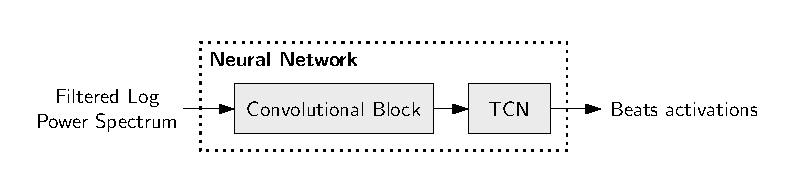
\includegraphics[scale=0.8]{figures/neural_net.eps}
\end{minipage}
\vspace{2em}

\begin{minipage}{\textwidth} 
\centering
\includegraphics[scale=0.5]{figures/spectrum_activations.pdf}
\end{minipage}
 
\end{frame}


\begin{frame}
\frametitle{Convolutional Block}
\begin{itemize}
\item 3 layers of 16 filters: 1st/2nd layer ($3\times3$), 3rd layer ($1\times8$)
\item Max pooling over ($3\times1$) in 1st and 2nd layer
\item Exponential linear unit (ELU), and dropout of rate $0.1$
\end{itemize}
\begin{minipage}{\textwidth} 
\centering
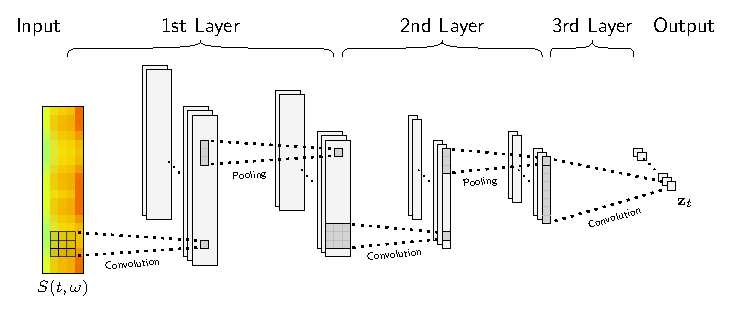
\includegraphics[scale=0.9]{figures/conv_block_color.eps}
\end{minipage}

\end{frame}


\begin{frame}
\frametitle{Filter Activation Maps}
\begin{figure}[htbp]
\centering
\begin{subfigure}[b]{0.4\textwidth}
\centering
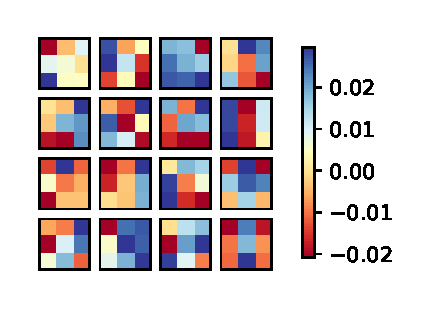
\includegraphics[scale=0.6]{figures/conv2d_layer_1.eps}
\caption{1st layer}
\end{subfigure}
~ %add desired spacing between images, e. g. ~, \quad, \qquad, \hfill etc. 
%(or a blank line to force the subfigure onto a new line)
\begin{subfigure}[b]{0.4\textwidth}
\centering
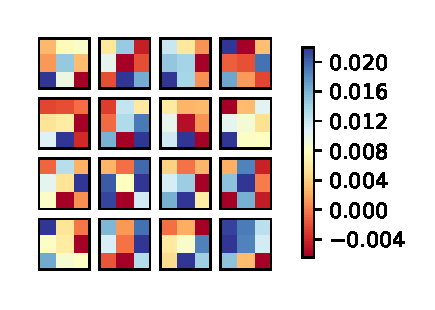
\includegraphics[scale=0.6]{figures/conv2d_layer_2.eps}
\caption{2nd layer}
\end{subfigure}
~ %add desired spacing between images, e. g. ~, \quad, \qquad, \hfill etc. 
%(or a blank line to force the subfigure onto a new line)
\begin{subfigure}[b]{0.9\textwidth}
\centering
\vspace{1em}
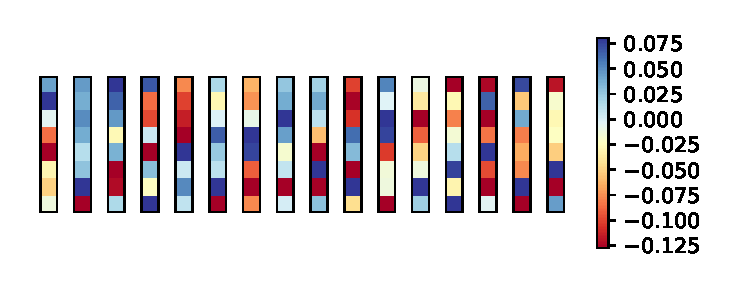
\includegraphics[scale=0.6]{figures/conv2d_layer_3.eps}
\caption{3rd layer}
\end{subfigure}
\end{figure}
\end{frame}



\begin{frame}
\frametitle{Temporal Convolutional Networks}
\begin{itemize}
\item  Dilated convolutions with filter $f:\{ 0, \dots, k-1\} \rightarrow \mathbb R$
\end{itemize}
\vspace{-0.5em}
\begin{align}
F(x) = (\mathbf x *_d f)(x) = \sum_{i=0}^{k-1} f(i) \, \mathbf x_{s-d\cdot i}
\end{align}
\vspace{-0.5em}
\begin{itemize}
% \item exponentially large receptive field
\item Dilation factor $d = 2^\nu$ with $\nu$ level, and $k$ filter size
\end{itemize}
\vspace{1em}
\begin{minipage}{\textwidth} 
\centering
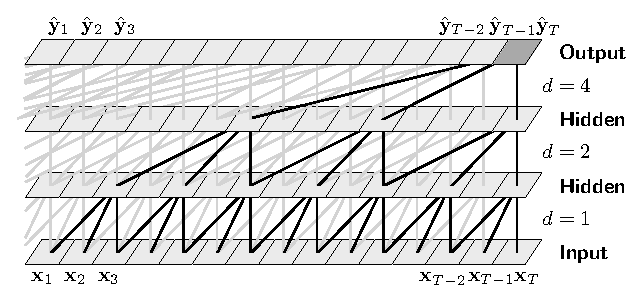
\includegraphics[scale=0.8]{figures/dilated_conv_full.eps}
\end{minipage}

\end{frame}


\begin{frame}
\frametitle{Residual Block}
\begin{minipage}{0.55\textwidth} 
\begin{itemize}
\item Residual connections: layers learn modifications $\mathcal F$ to the identity mapping rather than the entire transformation \cite{He2016}
\end{itemize}
\vspace{-0.5em}
\begin{align}
\hat{\mathbf z}^{(i)} = \hat{\mathbf z}^{(i-1)} + \mathcal F( \hat{\mathbf z}^{(i-1)})
\end{align}
\vspace{-1em}
\begin{itemize}
\item Weight normalization \cite{Salimans2016} and spatial dropout \cite{Srivastava2014} is applied to the filters
\item Enables stabilization for very deep networks
\end{itemize}
\end{minipage}
% \hfill
\hspace{-0.5em}
\begin{minipage}{0.4\textwidth} 
\centering
\vspace{-0.6em}
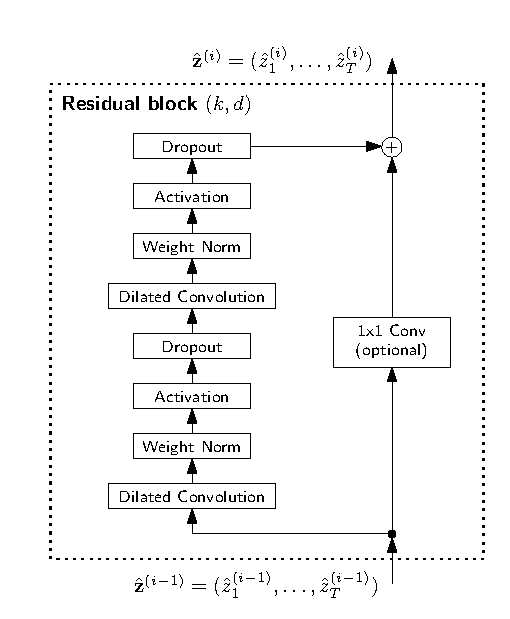
\includegraphics[scale=0.7]{figures/residual_block.eps}
\end{minipage}
\end{frame}



\begin{frame}
% \frametitle{Feature Learning}

\begin{minipage}{\textwidth} 
\centering
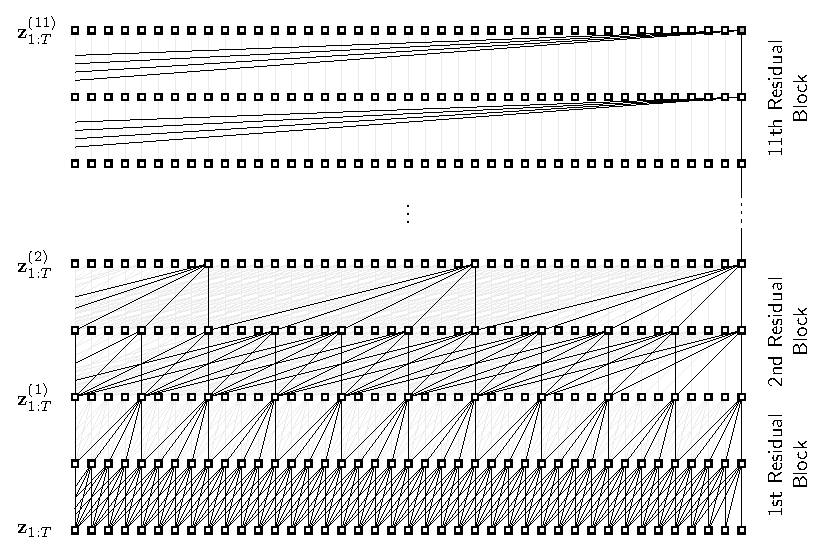
\includegraphics[scale=0.7]{figures/tcn.eps}
\end{minipage}
 
\end{frame}




\begin{frame}
\frametitle{Network Output}

\begin{itemize}
\item The output layer of the TCN is a fully-connected linear layer with two units, representing the classes ``beat'' and ``no beat''
\item Normalization of the output with the log softmax function 
% \begin{align}
% \log \text{softmax}(\hat{y}_i) = \log\left(\frac{\exp{(\hat{y}_i)}}{\sum_j \exp(\hat{y}_j)}\right)
% \end{align} 
\item The output $\hat{\mathbf y}_t = (\hat{y}_{1_t}, \hat{y}_{2_t})^T$ represents the log-probabilities for the two classes at time $t$.
\item The network can thus be trained as a binary classifier with the negative log likelihood loss function
\begin{align}
\label{eq:binary_cros_entropy_loss}
L(\mathbf y, \hat{\mathbf y}) = - w_0 \,y_0 \log(\hat{y}_0)-w_1\,y_1 \log(\hat{y}_1)
\end{align} 
\item The beat activations $a_{1:T}$ can be calculated by
\begin{align}
a_t = \exp \left({\hat{y}_{1_t}} \right), \quad \, t= 1,\dots,T
\end{align}  
\end{itemize}
\end{frame}


\begin{frame}
\frametitle{Network Training}
\begin{itemize}
\item Final model has ``only'' $\num[group-separator={,}]{30818}$ trainable parameters
\item Trained with ADAM optimizer \cite{Kingma2014} with standard parameters on 8 NVIDIA Tesla V100 GPUs in parallel
\item Hyperparameter search \cite{nevergrad}: Convergence is fastest with a batch size of $M = 80$ and an learning rate of $\mu = 5 \cdot10^{-3}$
\item Once the validation loss saturates, the learning rate is decreased to $10^{-5}$ in order to fine-tune the model
\end{itemize}
\begin{minipage}{\textwidth} 
\centering
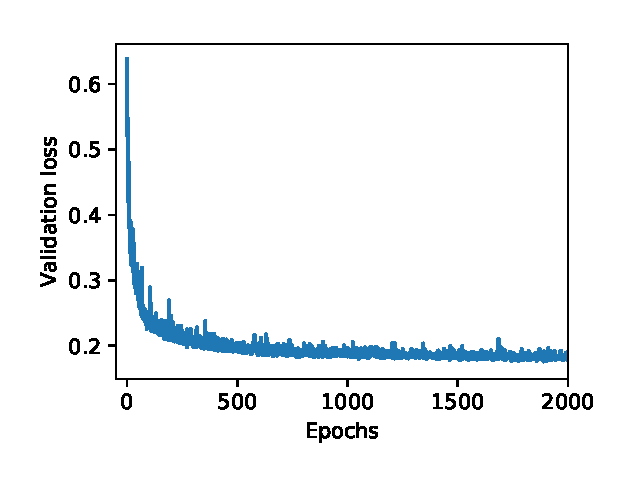
\includegraphics[scale=0.55]{figures/validation_loss.eps}
\end{minipage}
\end{frame}


\subsection{Temporal Decoding}

\begin{frame}
\frametitle{Temporal Decoding}

\begin{itemize}
\item The metrical structure is build upon a hierarchy of approximate regular pulses $\rightarrow$ use probabilistic dynamic model 
\item \textbf{Input}: Beat activations $a_t \in [0,1], \quad t = 1.\dots, T$
\end{itemize}

\begin{minipage}{\textwidth} 
\centering
\includegraphics[scale=0.5]{figures/activations.pdf}
\end{minipage}

\begin{itemize}
\item \textbf{Model}: Hidden Markov model (HMM) with hidden state
\begin{align}
\mathbf s_t = (\phi_t, \tau_t)^T
\end{align} 
with \textbf{phase} $\phi_t \in \{1, \dots, \tau_t\}$, and \textbf{period} $\tau_t \in \{ \tau_{\text{min}}, \dots, \tau_{\text{max}}\}$

\vspace{0.5em}
\item Tempo range from 55 to 215 BPM $\Rightarrow$  $\tau_\text{min} = 27$,  $\tau_\text{max} = 107$ 
\end{itemize}
\end{frame}




% Given a sequence of beat activations $a_{1:T}$, the goal of the hidden Markov model is to identify the most probable hidden state sequence $\mathbf s_{1:T}^*$. For every time frame $t$, the hidden state is defined as $\mathbf s_t = (\phi_t, \tau_t)^T$ where $\phi_t \in \{1, 2, \dots, \tau_t\}$ denotes the position inside a beat period, and $\tau_t \in \{ \tau_{\text{min}}, \dots, \tau_{\text{max}}\}$ refers to the length of the current beat period measured in frames. Due to the principle to use exactly one state per frame to indicate the position inside the beat period, the number of position states corresponds exactly to length of the current beat period $\tau_t$. Usually, the tempo $\Theta$ of a musical piece is measured in beats per minute (BPM), and therefore needs to be converted to the beat period measured in frames, by
% \begin{align}
% \tau(\Theta) = \left\lfloor \frac{\Theta}{60}\, f_r \right\rfloor 
% \label{eq:number_of_obstervations_per_bar}
% \end{align} 
% where the frame rate $f_r$ is defined as $100$ frames per second. The limits of the beat period can be easily obtained as $\tau_\text{min} = \tau(\Theta_\text{max})$ and $\tau_\text{max} =\tau(\Theta_\text{min})$ respectively. Operating on a tempo range from 55 to 215 BPM results in a beat period ranging from $\tau_\text{min} = 27$ to $\tau_\text{max} = 107$ frames, and thus constructs a state space with 5427 states in total. As an illustration, a toy example with a significantly smaller state space  is shown in Fig. \ref{fig:state_space}.


\begin{frame}
\frametitle{State Space}
\begin{itemize}
\item Phase $\phi_t \in \{1, \dots, \tau_t\}$: Position inside the beat period
\item Beat period $\tau_t \in \{ \tau_{\text{min}}, \dots, \tau_{\text{max}}\}$: Reciprocal of the tempo
\item Use exactly one state per frame to indicate the position inside the beat period
\item[$\Rightarrow$] State space with $5427$ states in total
\end{itemize}

\begin{minipage}{\textwidth} 
\centering
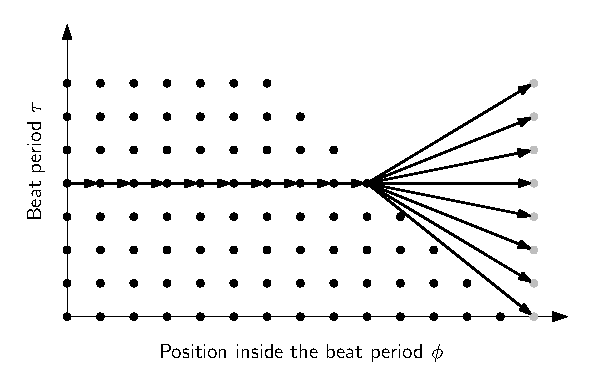
\includegraphics[scale=0.7]{figures/state_space.eps}
\end{minipage}

\end{frame}


\begin{frame}
\frametitle{Inference}

\begin{itemize}
\item Most likely hidden state sequence with Viterbi algorithm \cite{Viterbi1967}
\begin{align}
\mathbf s_{1:T}^* = \argmax_{\mathbf s_{1:T}} P(\mathbf s_{1:T}\,|\, a_{1:T})
\label{eq:most_likely_states}
\end{align} 
\vspace{-1.5em}
\begin{align}
 P(\mathbf s_{1:T}\,|\, a_{1:T}) \propto P(\mathbf s_1) \prod_{t=2}^T P(\mathbf s_t\,|\,\mathbf s_{t-1})\, P( a_t\,|\,\mathbf s_{t})
\end{align} 
\item Initial state distribution: $P(\mathbf s_1)$
\item Transition model: $P(\mathbf s_t\,|\,\mathbf s_{t-1})$ 
\item Observation model: $P(a_t\,|\,\mathbf s_{t})$
\vspace{1em}
\item \textbf{Initial Distribution}: Incorporate prior knowledge about tempo (uniform distribution $\Rightarrow$ all states are equiprobable)
\end{itemize}
\end{frame}



\begin{frame}
\frametitle{Hidden Markov Model}
\begin{itemize}
\item \textbf{Transition model:} Decompose into distributions for each of the two hidden variables
\begin{align}
P(\mathbf s_t\,|\,\mathbf s_{t-1}) = P(\mathbf \phi_t\,|\,\mathbf \phi_{t-1}, \tau_{t-1}) \, P(\tau_t \, |\, \tau_{t-1}) 
\end{align} 
\vspace{-1em}
\begin{align}
P(\mathbf \phi_t\,|\,\mathbf \phi_{t-1}, \tau_{t-1}) = \mathbf 1_A
\end{align} 
with the indicator function $\mathbf 1_A$ that equals one if $\phi_t = (\phi_{t-1}+\tau_{t-1}-1)\mod M+1$
\begin{align}
P(\tau_t \, |\, \tau_{t-1}) = \frac{\lambda}{2 \, \tau_{t-1}}\exp \left( -\lambda \left| \frac{\tau_{t}}{\tau_{t-1}} -1 \right| \right)
\end{align} 
\item \textbf{Observation model}:
\vspace{-0.5em} 
\begin{align}
P(a_t\,|\,\phi_t) = \begin{cases}
    a_t, &1 \leq \phi_t\leq \frac{\lambda}{\Lambda}\\
    \frac{1-a_t}{\lambda-1}, &\text{else}.    
\end{cases}
\end{align} 

\end{itemize}



% \paragraph{Transition Model} The transition model $P(\mathbf s_t\,|\,\mathbf s_{t-1})$ can be further decomposed into a distribution for each of the two hidden variables $\phi_t$ and $\tau_t$, this is
% \begin{align}
% P(\mathbf s_t\,|\,\mathbf s_{t-1}) = P(\mathbf \phi_t\,|\,\mathbf \phi_{t-1}, \tau_{t-1}) \, P(\tau_t \, |\, \tau_{t-1}) 
% \end{align} 
% where the first factor is defined as
% \begin{align}
% P(\mathbf \phi_t\,|\,\mathbf \phi_{t-1}, \tau_{t-1}) = \mathbf 1_A
% \end{align} 
% with the indicator function $\mathbf 1_A$ that equals one if $\phi_t = (\phi_{t-1}+\tau_{t-1}-1)\mod M+1$. The modulo operator makes the bar position cyclic. If $\phi_t = \tau_t$, the second factor is defined by a Laplace distribution
% \begin{align}
% P(\tau_t \, |\, \tau_{t-1}) = \frac{\lambda}{2 \, \tau_{t-1}}\exp \left( -\lambda \left| \frac{\tau_{t}}{\tau_{t-1}} -1 \right| \right)
% \end{align} 
% otherwise it is
% \begin{align}
% P(\tau_t \, |\, \tau_{t-1}) = \begin{cases}
%     1, &\tau_t = \tau_{t-1}\\
%     0, &\text{else.} 
% \end{cases}
% \end{align} 

\end{frame}

\section{Evaluation}

\begin{frame}
\frametitle{Evaluation Methods}

\begin{itemize}
\item \textbf{Input}: Set of annotated beat times $\mathcal A = \{a_1, \dots, a_A\}$ and a corresponding set of predicted beat times $\mathcal B = \{b_1, \dots, b_B\}$
\item \textbf{F-measure}: A detected beat is regarded as true positive if it is in $\pm 70\,\text{ms}$ range of an annotated beat
\begin{align}
F_1= \dfrac{2\, tp}{2\, tp + fp + fn}
\end{align} 
\item \textbf{Continuity measures}: Number of correct beats in each continuously correct segment $Y_m$
\begin{align}
\text{CML}_\text{c} = \frac{\max(Y_m)}{A}, \quad
\text{CML}_\text{t} = \frac{\sum_{m=1}^MY_m}{A},\quad
\end{align} 
$\text{AML}_\text{c}$ and $\text{AML}_\text{t}$ allow double or half the correct metrical level
\item \textbf{Information Gain}: Measure of how much information the beats provide about the annotations \cite{Davies2009b}
\end{itemize}
\end{frame}



\begin{frame}
\frametitle{Results}
\begin{itemize}
\item The achieved performance is compared against the state-of-the-art beat tracker Madmom \cite{Boeck2014}
\end{itemize}
\begin{table}[htbp]
\tiny
\centering
%% local redefinitions 
\sisetup{table-align-uncertainty=true,separate-uncertainty=true,}
\renewrobustcmd{\bfseries}{\fontseries{b}\selectfont}
\renewrobustcmd{\boldmath}{}
\begin{tabular}{lcccccc}
\hline \hline
& F-Measure & CMLc & CMLt & AMLc & AMLt & D
\vspace{0.0em}\\\hline \vspace{-1.5em}
\csvreader[head to column names, filter equal={\dataset}{1}]{/Users/juliusrichter/Documents/Uni/Masterarbeit/beat_tracker/data/performance.csv}{}
{\\\name & \Fmeasure & \CMLc & \CMLt & \AMLc & \AMLt & \D}
\vspace{0.2em}\\\hline \vspace{-1.5em}
\csvreader[head to column names, filter equal={\dataset}{2}]{/Users/juliusrichter/Documents/Uni/Masterarbeit/beat_tracker/data/performance.csv}{}
{\\\name & \Fmeasure & \CMLc & \CMLt & \AMLc & \AMLt & \D}
\vspace{0.2em}\\\hline \vspace{-1.5em}
\csvreader[head to column names, filter equal={\dataset}{3}]{/Users/juliusrichter/Documents/Uni/Masterarbeit/beat_tracker/data/performance.csv}{}
{\\\name & \Fmeasure & \CMLc & \CMLt & \AMLc & \AMLt & \D}
\vspace{0.2em}\\\hline \vspace{-1.5em}
\csvreader[head to column names, filter equal={\dataset}{4}]{/Users/juliusrichter/Documents/Uni/Masterarbeit/beat_tracker/data/performance.csv}{}
{\\\name & \Fmeasure & \CMLc & \CMLt & \AMLc & \AMLt & \D}
\vspace{0.2em}\\\hline \hline
\end{tabular}
\end{table}

\end{frame}


\section{Examples}

\begin{frame}
\frametitle{Examples}
From dataset:
\begin{itemize}
\item Joss Stone - Torn and Tattered (SMC dataset)  \\ 
$\rightarrow$ Pop music, very easy to track the beat (100$\%$ accuracy)
\item Led Zeppelin - The Crunge (GTZAN dataset) \\ 
$\rightarrow$ Rock music, with change of meter
\item William Byrd - Mass For Four Voices (Hainsworth dataset) \\ 
$\rightarrow$ Choral music, no percussion, not easy to track the beat
\end{itemize}
Unseen data:
\begin{itemize}
\item Kimio Eto - Yuki No Genso  \\ 
$\rightarrow$ Traditional Japanese Koto with expressive timing \\\vspace{0.5em}
(Presentation with 808-Beat in Ableton Live)
\end{itemize}

\end{frame}


\begin{frame}
\frametitle{Joss Stone - Torn and Tattered (SMC dataset)}
\begin{minipage}{\textwidth} 
\centering
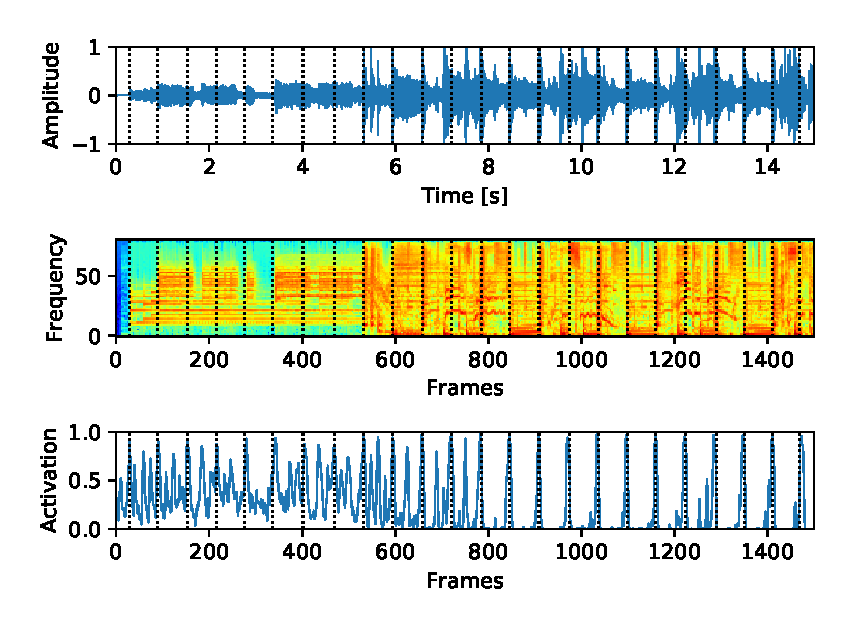
\includegraphics[scale=0.6]{figures/joss_stone.eps}
\end{minipage}
\end{frame}


\begin{frame}
\frametitle{Led Zeppelin - The Crunge (GTZAN dataset)}
\begin{minipage}{\textwidth} 
\centering
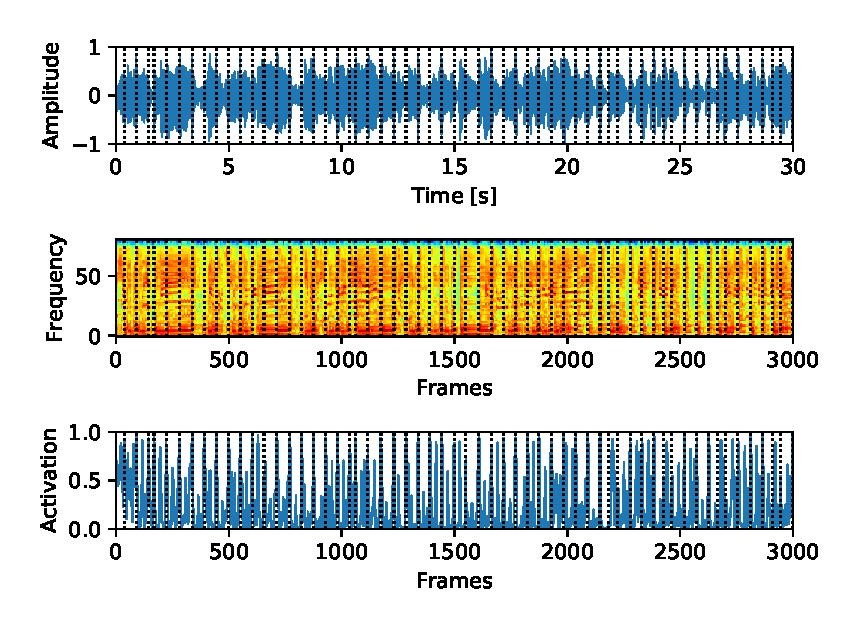
\includegraphics[scale=0.6]{figures/led_zeppelin.eps}
\end{minipage}
\end{frame}


\begin{frame}
\frametitle{William Byrd - Mass For Four Voices (Hainsworth dataset)}
\begin{minipage}{\textwidth} 
\centering
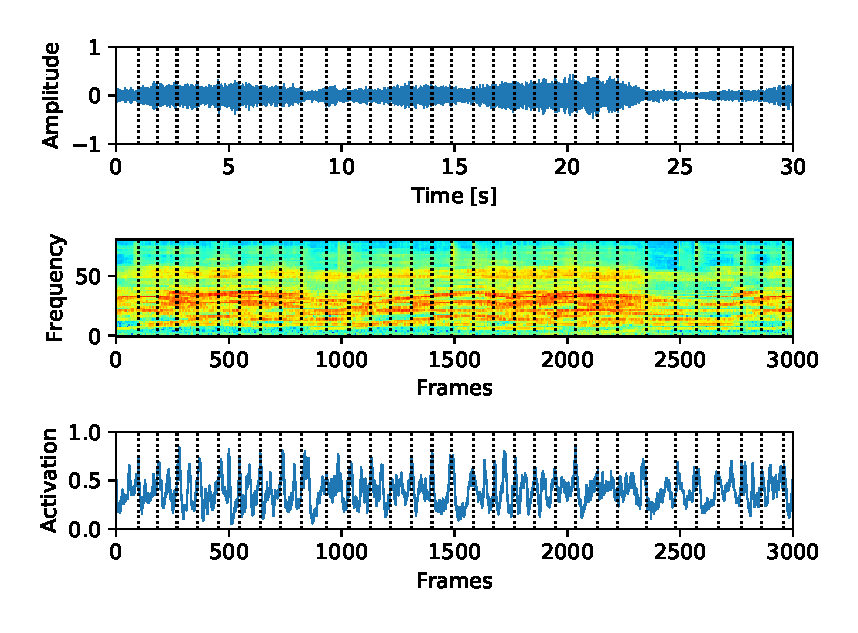
\includegraphics[scale=0.6]{figures/Tallis_Scholars.eps}
\end{minipage}
\end{frame}



\begin{frame}
\frametitle{Kimio Eto - Yuki No Genso}
\begin{minipage}{\textwidth} 
\centering
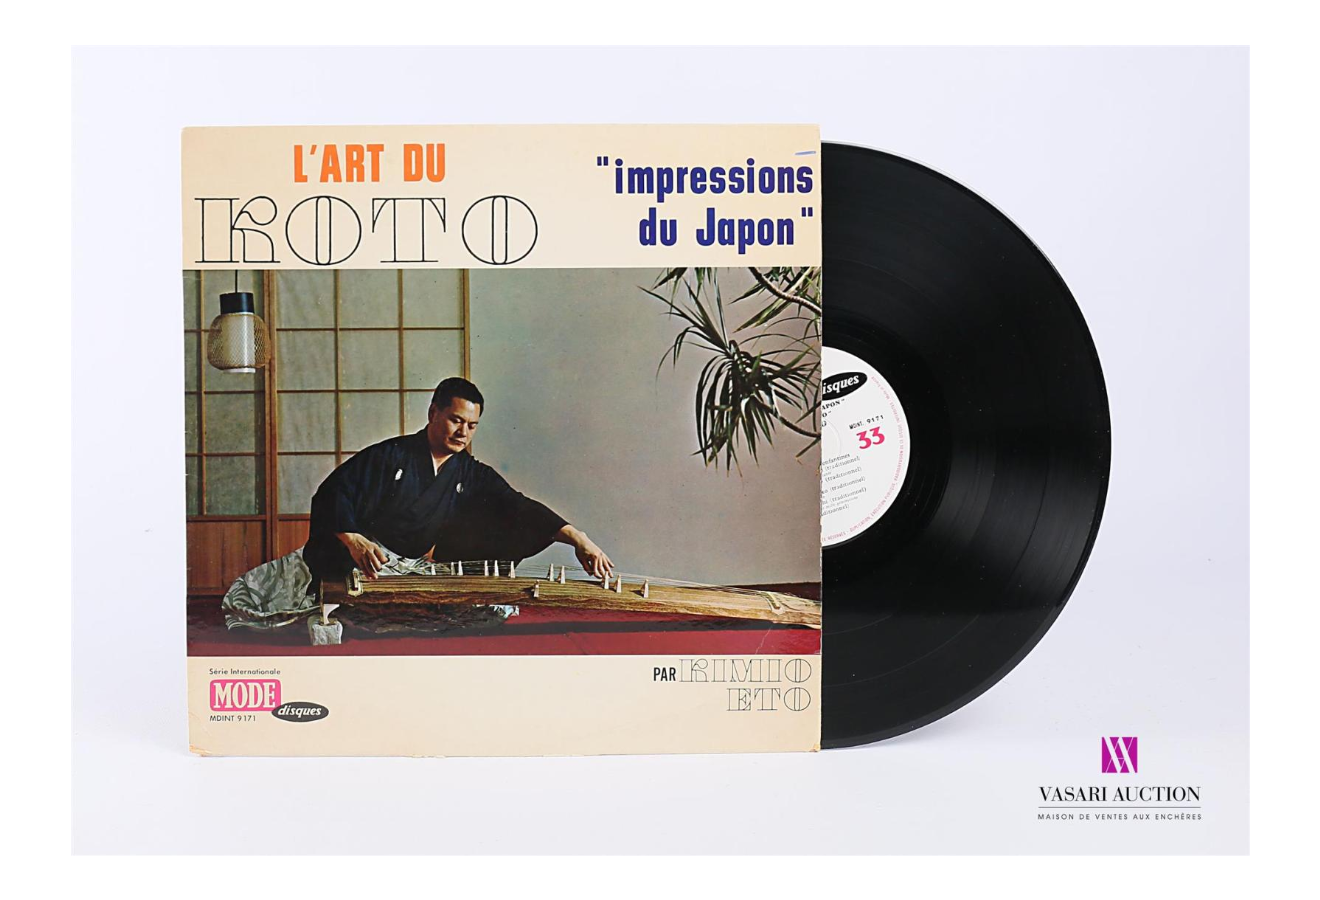
\includegraphics[width=\textwidth]{figures/l'art_du_koto.png}
\end{minipage}
\end{frame}




% \begin{frame}
% \frametitle{Ca Trù - Traditional Vietnamese}
% \begin{minipage}{\textwidth} 
% \hspace{-2em}
% 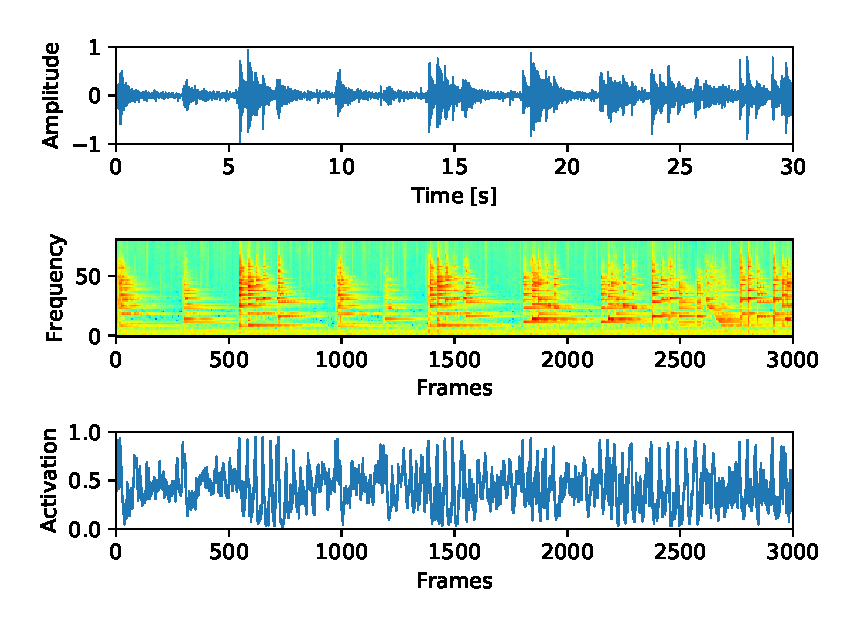
\includegraphics[scale=0.6]{figures/ca_tru.eps}
% \end{minipage}
% \end{frame}




\section{Conclusion}

\begin{frame}
\frametitle{Conclusion}
\begin{itemize}
\item Computational beat tracking system for musical audio, that uses convolutional neural networks to learn the beat activation as a high-level feature directly from the preprocessed audio
\item A dynamic Bayesian network is used to model beat periods of various lengths and align the predicted beat positions to the best global solution
\item Compared against a current state-of-the-art beat tracker, the proposed approach maintains \textbf{competitive performance} but with two distinct computational advantages. It works \textbf{causally} and requires considerably \textbf{less learnable parameters}. 
\end{itemize}
\end{frame}



\begin{frame}
\frametitle{Future Research}
\begin{itemize}
\item Investigate different model architectures (e.g. deep equilibrium models \cite{Bai2019b})
\item Leave high-level rhythmical analysis solely to the neural network 
\item Instead of preprocessing the audio signal with the STFT, let the network automatically learn an intermediate representation
\item Utilize a multi-task learning strategy (e.g. incorporate the basic tempo as additional annotation \cite{Boeck2019})
\item Real-time implementation of the beat tracking system
\item Participate at the MIREX beat tracking contest 2019
\end{itemize}
\end{frame}




% The connection to practical settings, however, still remains elusive





\frame[plain]{
% \color{black}
% \hspace*{-2.85em}
% \vrule height\paperheight width\paperwidth%
\centering
Thank you for your attention.
}

\section*{Additional slides}


\begin{frame}[noframenumbering, allowframebreaks] % Quellenverzeichnis über mehrere Folien
\frametitle{References}

\setbeamertemplate{bibliography item}[text]
% \bibliographystyle{literatur/unsrtdin.bst}
\bibliographystyle{unsrt}
% \nocite{*} % Alle Referenzen ins Quellenverzeichnis aufnehmen
\tiny
\bibliography{References}

\end{frame}


\begin{frame}
\frametitle{History of Beat Tracking}
% \begin{itemize}
% \item One key principle of interference managment is treating interference as noise (TIN) 
% \end{itemize}
\begin{itemize}
% \event{1985}{Schloss \cite{Schloss1985}}
% \event{1990}{Allen and Dannenberg \cite{Allen1990}}
% \event{1994}{Goto and Muraoka \cite{Goto1994}}
% \event{1998}{Scheirer \cite{Scheirer1998}}
% \event{2001}{Cemgil et al. \cite{Cemgil2001}, Dixon \cite{Dixon2001}}
% \event{2003}{Laroche \cite{Laroche2003}}
% \event{2005}{Klapuri et al. \cite{Klapuri2005}}
% \event{2007}{Davies and Plumbley \cite{Davies2007}}
% \event{2009}{Peeters \cite{Peeters2009}}
% \event{2011}{Böck and Schedl \cite{Boeck2011}}
% \event{2014}{Böck et al. \cite{Boeck2014}}
% \eventmarker{2015}{Krebs et al. \cite{Krebs2015}}
% \eventlabel{2016}{Krebs et al. \cite{Krebs2015}}
% \event{2019}{Davies and Böck \cite{Davies2019}}
\item[1985] Schloss \cite{Schloss1985}: Onset detection by observing peaks the amplitude envelope. Beat period is inverse of the lowest frequency.
\item[1994] Goto and Muraoka \cite{Goto1994}: Multiple agents detect hits of bass drum and snare drum.
\item[2001] Cemgil et al. \cite{Cemgil2001}: Formulate beat tracking in a probabilistic Bayesian framework where tempo and beat is modeled as a stochastic dynamical system.
\item[2011] Böck and Schedl \cite{Boeck2011}: First beat tracking system based on recurrent neural networks (RNNs).
\item[2014] Böck et al. \cite{Boeck2014}: Multiple recurrent neural networks are used, which are trained on certain heterogeneous music styles
\item[2019] Davies and Böck \cite{Davies2019}: Suggest to use a convolutional neural network in the form of a temporal convolutional network 
\end{itemize}
\end{frame}


\begin{frame}
\frametitle{Sequence to Sequence Modeling}
\begin{itemize}
\item \makebox[8em]{Input sequence\hfill}  $\mathbf x_{1:T} := \mathbf x_1, \dots, \mathbf x_T$ 
\vspace{0.5em}
\item \makebox[8em]{Output sequence\hfill} $\mathbf y_{1:T} := \mathbf y_1, \dots, \mathbf y_T$ 
\vspace{0.5em}
\item \makebox[8em]{Sequence model\hfill} $f: \mathcal X^T \rightarrow \mathcal Y^T$ \\\vspace{0.5em}(here: $\mathcal X = \mathbb R^{88}, \mathcal Y = \mathbb R^2$)
\end{itemize}
\begin{align}
\mathbf y_1, \dots, \mathbf y_T  = f(\mathbf x_1, \dots, \mathbf x_T)
\end{align}
\begin{itemize}
\item The input  $\mathbf x_t \in \mathbb R^{88}$ to the neural network corresponds to the frequency column of the filtered log power spectrogram
\end{itemize}
\begin{align}
\mathbf x_t = S(t,\omega), \quad \forall\, t= 1,\dots,T
\end{align}
\end{frame}



\end{document}


